% chap3.tex (Definitions and Theorem)

\chapter{Sensor Data Provenance Collection Framework for the IoT}

In this chapter, we define how provenance is collected and modeled along the IoT architectural stack. We also define implementation specifics of our provenance collection framework. 

\section{IoT Provenance-Collection framework Information flow}
%This section discusses the data model in which we represent sensor and actuator reading of provenance data collected from IoT devices . It also talks about the relationship between IoT provenance Collection and PROV\-DM; How data is process and dissemenated accross the IoT architecture.
%
%\textcolor{red}{TODO: Talks about how we use PROV\-DM and what kinds of provenance we are looking to store}

A provenance model is used to represent causal dependency between objects and it is usually modeled as a Directed Acyclic Graph(DAG). This enables for better graphical representation of provenance relationships and also a unified format for representing provenance data. There are two major models for representing provenance, OPM and Prov-DM. PROV-DM is a predecessor and standardized version of OPM. It allows the modeling of data objects either physical or digital. PROV-DM is chosen as the model to represent provenance for our implementation because it allows for proper representation of all of the relationships in which we envision for IoT devices. This section defines a model for relaying provenance in IoT systems which is built on top of PROV-DM. 
From the IoT architecture as illustrated in Section 2, data is disseminated from sensors and actuators across various layers contained in the IoT architectural stack. The provenance data produced from various sensors and actuators are collectively aggregated at the gateway layer and/or the cloud layer. We allow for provenance data to be translated to PROV-DM format at the various levels of the IoT architecture. This allows offline processing of information at all layers of the IoT architecture even in the case of a network failure. Sensor readings are collected from devices as specified by a policy. Policy specifications help address the issue with memory constraint  of collecting provenance data in IoT devices. Policy specification and implementation are discussed in greater detail in chapter 4.  Figure 4.1 illustrates the provenance data aggregation that occurs at various layers of the IoT architectural stack. Data is collected from sensors and actuators and collectively aggregated and passed across the various hierarchies contained in the IoT architecture. 


\begin{figure}[h!]
\begin{center}

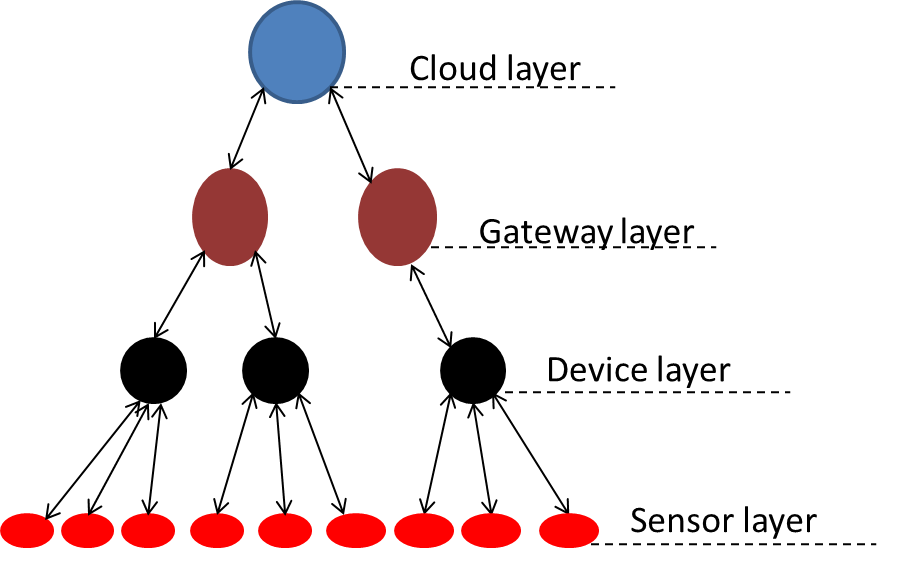
\includegraphics[width=3.0in]{iot.PNG}    
\end{center}
\caption{IoT provenance-collection data aggregation}
\label{autom}
\end{figure}


Using the scenario of a smart home use case as illustrated in chapter 2, a detailed example of how our provenance collection framework can be applied is described as follows:

\begin{itemize}

\item Provenance data is collected from sensor and actuator readings of devices contained in the smart home(e.g thermostat, refrigerator, and smart doors). The provenance data is collected as specified in a policy document. Policy document contains information of which provenance data to be collected in the device and can be only be defined by the device owner who serves as an administrator. 

\item Provenance data from multiple sensor and actuator readings collected from each device is aggregated and passed along to the gateway. THis information is transmitted to the cloud for storage in which further analysis could be conducted on the data to derive insights from the provenance data collected. This information is then transferred to the cloud for long term storage. Each layer in the provenance IoT architecture is independent of the and maintains provenance information that can be mapped using the PROV\-DM format which allows for the representation of dependencies that exists between objects contained in the device. This allows for provenance data to be further analyzed offline at the respective layers even in an event of network loss. 

\end{itemize}





\subsection{Provenance-Collection Model Definition}

It is assumed that provenance data is collected from the underlying IoT device using the framework outlined in section 3 of this chapter. Data is collected from sensors and actuators attached to an IoT device. The underlying construct is represented as a acyclic graph which denotes the relationship between multiple sensors and actuator readings. Since PROV-DM type provides a generic model for relaying provenance information, we define a more specific construct for representing provenance data in IoT devices based on  PROV-DM. In the context of IoT provenance, entity, process and agent are defined as follows:

\begin{itemize}

\item Agent: An agent contains information on an object that accesses an entity. Examples of agents in an IoT architecture are sensors, actuators, user roles(e.g admin). A unique identifier is given to each agents contained in an IoT framework.

\item Entity:  An entity can be defined as a data object that contains information which can be modifiable. An example entities are device files, processes, device memory contents.

\item Activity: An activity is a modification that an agent makes on an entity. An example of an activity are basic file access operations such as read, write, delete, update. 


\end{itemize}


To better emphasize the provenance-collection model, an example of a use case is illustrated in the figure below.



\begin{figure}[h]
\begin{center}

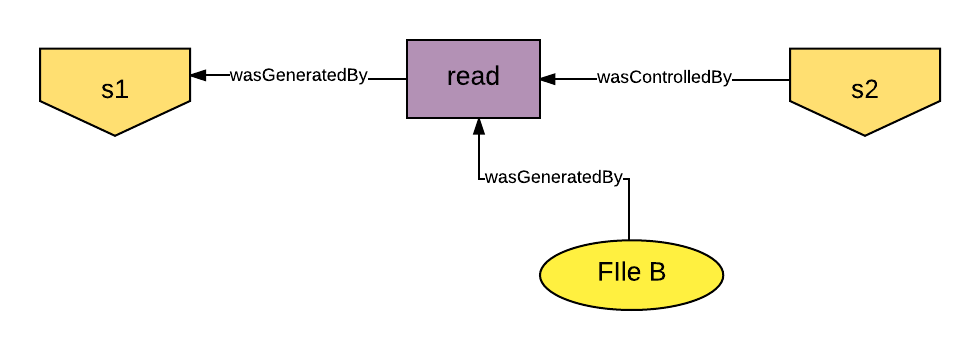
\includegraphics[width=4.0in]{provenance_model.png}    
\end{center}
\caption{Provenance-model use case}
\label{autom}
\end{figure}





The figure above depicts a dependency relationship between two sensors, s1 and s2. Consider the scenario of a smart home. s1 is smart thermostat contained in a smart home which regulates the temperature of the home and s2 is a sensor that detects the outside temperature. s1 constantly checks the temperature outside to regulate the temperature of the house accordingly. s1 tries to access information from s2. According to the provenance data model  definition, s1 and s2 are agents. The activity performed on s2 by s1 is read. File B is the entity in which s1 tries to read from s2 to determine the environmental temperature. The relationship between various components contained in the model is illustrated on the edges of the graph.

\par The relations define the relationship between types of a provenance model. We use the same instance of the relations contained in PROV-DM to represent relationships between types contained in the IoT framework.


\section{Provenance-Collection System}

In this section, we outline the components of our system and describe how provenance trace is collected across the IoT framework. Figure 1 displays the system architecture of our approach. Sensor and actuator readings in the form of Input and output(I/O) trace are recorded by the tracer component. This component intercepts system level I/O events and produces trace information in Common Trace Format (CTF). CTF represents binary trace output information containing multiple streams of binary events such as I/O activity. Trace information is converted into the PROV-DM and serialized to PROV-JSON. This represents the relationship between provenance entities contained in the system. CTF conversion to PROV-DM will be achieved using babeltrace. Babeltrace is a plugin which allows the conversion of CTF trace into various readable format. It includes plugins in which CTF trace data can be intercepted to create a custom conversion format. Our system relies heavily on data pruning to reduce and remove unimportant provenance data in order to conserve memory and address the memory constraint issues faced by low memory embedded systems. This is achieved by using a policy in which a user with administrative privilege is given permission to create or modify a policy. This policy document dictates what provenance data to collect. Pruned provenance from the device is securely transmitted to a gateway and later transmitted and stored in a private cloud backend. The backend of choice is Neo4j, a graph database for efficient storage, query and visualization of provenance data.

\begin{figure}[h]
\begin{center}

\includegraphics[width =3.0in]{architecture.PNG}    
\end{center}
\caption{Proposed Model}
\label{architecture}
\end{figure}

The goal is to create a provenance\-aware system which records I/O operations on data for devices connected in an IoT system. For our implementation, several tools and hardware components are utilized in the development of our prototype, some of the tools utilized are outlined below:

\begin{itemize}
\item BeagleBone Black Board. This device is a microcontroller used to evaluate our approach. We choose the BeagleBone Board because it is a representation of what can be found on an IoT gateway device and it has the capability to include custom hardware in programmable logic. Also, BeagleBone is a low cost, simple IoT demonstrator that was chosen for its high performance, on­board emulation, and IoT gateway projects can be programmed without additional need for hardware tools.

%\item Real Time Executive for Multiprocessor Systems (RTEMS) is an open source real­time operating system (RTOS) for embedded systems. This operating system is a typical RTOS that may be deployed in IoT devices.

\item Neo4j, a graph database which allow optimized querying of graph data. Since provenance represents causal dependencies, it is ideal to use a graph database to store the relationships between objects

\item lttng, a software tool for collecting system level trace on Linux system. 

\end{itemize}


\section{Experiment Evaluation}

I plan to evaluate the effectiveness of my approach for provenance collection by using an intrusion detection system specifically developed for IoT. An IDS is used to detect malicious attacks based on certain policy or threshold specified by an administrator. There are two types of  IDS: rule-based/Signature-based approach, and anomaly-based approach. Signature-based approach allows for intrusion monitoring by specific known signatures of malicious attacks. An example of a signature-based IDS is an anti-virus software. On the other hand, anomaly-based IDS monitors intrusion by patterns that falls out of the normal system function. Most anomaly-based approach deals with the use of machine learning to classify normal or anomalous behavior. This can be useful to detect unknown malicious attacks. Provenance collection IDS system uses provenance data to provide intrusion detection capabilities in an IoT framework. It follows a Signature-based approach in which provenance data collected from the IoT framework is used for intrusion detection. 
\par The IDS is developed using the work of Xie et al \cite{Xie:2016:UID:2936026.2936232}. Xie et al proposed an intrusion detection system, Provenance-aware Intrusion Detection and Analysis System(PIDAS). This system uses system-level provenance data to provide real-time vulnerability intrusion detection on system behaviors. The system collects provenance from system calls, detects intrusion and analyzes vulnerabilities that exists based on provenance data. PIDAS contains three essential components: the collector which records provenance information of applications running in the user space. Provenance data is stored in a key-value pair database for easy query of acyclic graphs. The detector extracts dependency relationships from the provenance data and stores this information in a repository for further analysis. The analyzer is responsible for identifying all other intrusion activities that might have occurred. It achieves this by making queries to view all dependencies from the detected intrusion point. Provenance detector is made possible by using a provenance-based algorithm that matches the path contained in the graph.


The detector consists of three steps. Rule-buit which collects normal system behavior of provenance data and stores this information in a ruleDB. A ruleDB consists of a key-value pair which has parent and child relationships in the dependency graph. The rule-built is used to match observed provenance events  to detect system intrusion. Provenance information in the form of a dependency relationship is matched with the child/parent dependency rule information contained in the ruleDB. This information is used to compute the decision value which determines if there has been an intrusion.  A description of the rule matching and scoring algorithm is described in detail below: 

\begin{itemize}

\item provenance data is divided into dependency relationships, $Dep_1,...,Dep_n. Dep_i =(A, B)$. Where A is the parent of B

\item The algorithm checks if there exists a match in the path between edges contained in the provenance dependency database, ruleDB. If there exists a path, a score of 1 is given to the path. This score is known as the path dubiety. Otherwise, if the path does not match any edge in the ruleDB, a score of 0 is given to the path.

Let R = provenance information of a program and G = provenance information contained in ruleDB. For each $Dep_i = (A, B) \in R, if Dep_i = (A, B) \in G$. intrusion dubiety = 1 else set intrusion dubiety = 0

\item The path decision, P is the sum of the dubiety of all the edges contained in the provenance data divided by the number of paths contained in the provenance dependency database.

 \[P =\frac{\sum\limits_{i=1}^W dubeity of Dep_i }{W} \] This information is compared with a threshold value, T. If P $>$ T, an anomaly exists in the system.

\end{itemize}

I plan to compare the integration of our provenance collection framework and storage efficiency framework with PIDAS with a baseline which consists of the PIDAS system without the integration of our proposed framework. More specifically, I plan to evaluate the false negative and false positive rate for the IDS system as compared with the baseline. False positive dictates the number of times in which an intrusion has been wrongly detected. This signifies that a path contained in an applications provenance was detected and not found in the ruleDB. On the other hand, false negative rate identifies the number of times a intrusion has not been detected. I also plan to evaluate the throughput of the system with the proposed baseline.





%\section{Provenance Aware IDS System for IoT }
%
%This section outlines the core functionalities of our model PAIST. 
